In this section we define the attacker model and show the security guarantees given by \lang. Specifically, we show that \lang{} executions satisfy termination-insensitive noninterference \cite{4223226}. Formally, an attacker is some principal $\Attacker$. Note that this principal might be a conjunction of named principals $n_1 \wedge \dots \wedge n_k$ representing a set of $k$ colluding principals. In the sections that follow we denote a $\Nameset$-indexed set of memories as a function $\globalstore: \Nameset \to (\Addr \to \val)$.

\subsection{Trace semantics}
We express the attacker model in terms of a trace semantics, in which certain operations in the language emit \emph{events} which are may or may not be observable by $\Attacker$. The grammar for events is given in Figure~\ref{fig:event-syntax}. These event should be self-explanatory, with the exception of $\mathsf{release}$ events, which we explain in Section~\ref{sec:release-events}. An non-empty event $\event$ contains the type of the event, the current environment when the event was emitted, and the node that emitted the event. An attacker observes modifications to memory (ie., writes an allocations) locally on a machine and remote procedure calls and returns across machines. This choice correspond to a typical Dolev-Yao attacker model \cite{Dolev:1981:SPK:1382435.1382728}.

\begin{figure}
\centering
\begin{align*}
\event &::= (\alpha, \env, n) \mid \varepsilon\\
\alpha &::= \mathsf{write}(\addr, \expr) \mid \mathsf{new}(\addr, \expr) \mid \mathsf{call}(\expr, n) \\ &\quad \mid \mathsf{ret}(\val, n) \mid \mathsf{stop}(\val, n) \mid \mathsf{release}(p, q, r)
\end{align*}
\caption{The syntax of events.}
\label{fig:event-syntax}
\end{figure}

We call a sequence of events a trace. We write the concatenation of traces as $t_1 \cdot t_2$ and we write the empty trace as $\varepsilon$. Given a trace $t$ the observable trace of $t$ is the trace $t \upharpoonright A$, defined as
\begin{align*}
\varepsilon \upharpoonright A &= \varepsilon\\
((\alpha, \env, n) \cdot t) \upharpoonright A &=
\begin{cases}
(\alpha, \env, n) \cdot (t \upharpoonright A) & \nopostflowstoquery{n; \env}{\env_n.\lblkw}{A} \\
t \upharpoonright A & \text{otherwise}
\end{cases}
\end{align*}

We augment the semantics from Section~\ref{sec:calculus} with events. Figure~\ref{fig:event-semantics} shows an excerpt of the augmented semantics. Except for the emitted event these rules correspond exactly to the rules in Figure~\ref{fig:monadic-reductions} and Figure~\ref{fig:global-steps}. It will be convenient to write $\gconfig{n}{\env}{S} \gstepstos[][t]$ when there exists a configuration $\gconfig{n'}{\env'}{S'}$ such that $\gconfig{n}{\env}{S} \gstepstos[][t] \gconfig{n'}{\env'}{S'}$. We also write $\gconfig{n}{\env}{S} \gstepstos[][\Attacker \filtertrace t']$ when $\gconfig{n}{\env}{S} \gstepstos[][t]$ and $t' = A \upharpoonright t$.

\begin{figure}
\centering
\begin{mathpar}
\inferrule[E-Write-Ev]{\store(\addr) = \lb{p}{\expr} \and \flowstoquery{n; \env}{\env_n.\lblkw}{p \flowsto n}{\level} \\\\ \nopostflowstoquery{n; \env}{\env_n.\lblkw \join \level}{n} \and \store' = \extend{\store}{\addr}{\lb{p}{\expr'}} \\\\ \sigma = \extend{\env_n}{\lblkw}{\env_n.\lblkw \join \level} \\\\ \event = (\mathsf{write}(\addr, \expr'), \env, n)}{\step{n; \env}[][\event]{\config{\store}{\efill{\writeref{\addr}{\expr'}}}}{ \config{\store'}{\efill{\return{()}}}}{\sigma}}
\and
\inferrule[G-Step-Ret-Ev]{S_n = \config{\store_n}{\efill{\wait{m}[\type]}} \and S_m = \config{\store_m}{\val ; \overline{\expr_m}} \\\\ \event = (\mathsf{ret}(\val, n), \env, m)}{\gconfig{m}{\env}{S} \gstepsto[][\event] \gconfig{n}{\env}{\extends{S}{n \mapsto \config{\store_n}{\efill{\val}}, m \mapsto \config{\store_m}{\overline{\expr_m}}}}}
\and
\inferrule[G-Step-Local-Ev]{\step{n; \env}[][\event]{S_n}{S'}{\sigma}}{\gconfig{n}{\env}{S} \gstepsto[][\event] \gconfig{n}{\extend{\env}{n}{\sigma}}{\extend{S}{n}{S'}}}
\and
\inferrule[E-Assume-Ev]{
\flowstoquery{n; \env}{\env_n.\lblkw}{r \flowsto n}{\level_1} \\\\ \actsforquery{n; \env}{\env_n.\lblkw}{\voice{q}}{\level_2} \\\\ \nopostflowstoquery{n; \env}{\env_n.\lblkw \join \level_1 \join \level_2}{n} \\\\ \sigma = \extends{\env_n}{\scope \mapsto \cons{\lb{r}{(p, q)}}{\env . \scope}), \lblkw \mapsto \env_n.\lblkw \join \level_1 \join \level_2} \\\\ \event = (\mathsf{release}(p, q, r), \env, n)}{\step{n; \env}[][\event]{\config{\store}{\efill{\adddelegate{p}{q}{r}}}}{ \config{\store}{\efill{\return{()}}}}{\sigma}}
\end{mathpar}
\caption{Augmented semantics emitting events.}
\label{fig:event-semantics}
\end{figure}

\paragraph{Release events}\label{sec:release-event}
In order to define noninterference we require that nodes agree on which principals flow to $\Attacker$. That is, it must not be the case that Alice considers data to not be observable by $\Attacker$, and then send it to Bob, who considers the same data to be observable by $\Attacker$. Relaxations of such limitations, like robust declassification \cite{???} and nonmalleable information-flow \cite{???}, is orthogonal to this work and therefore we consider only the case where nodes agree on which principals flow to $\Attacker$ in the information-flow lattice. To capture this intuition we introduce the notion of a ``good'' release event.

We call a release event $\event = (\mathsf{release}(p, q, r), \env, n)$ good, written $\good{A}{\event}$, if $\nopostflowstoquery{n; \env}{r}{A}$ implies $\nopostflowstoquery{n; \env}{p}{A} \iff \nopostflowstoquery{n; \env}{q}{A}$. Intuitively, this means that any expression of the form $\adddelegate{p}{q}{r}$ such that $r$ flows to $\Attacker$ should not modify what the attacker can observe. An illustration capturing when a flow is not good is shown in Figure~\ref{fig:bad-release}. We extend thie notion of good to traces and say a trace is good, written $\good{A}{t}$ if all release events in $t$ are good release events. Our noninterference result, presented in Section~\ref{sec:noninterference}, will quantify only over good traces, and we leave the problem of extending this result to more relaxed notions of noninterference as future work.

\begin{figure}
    \centering
    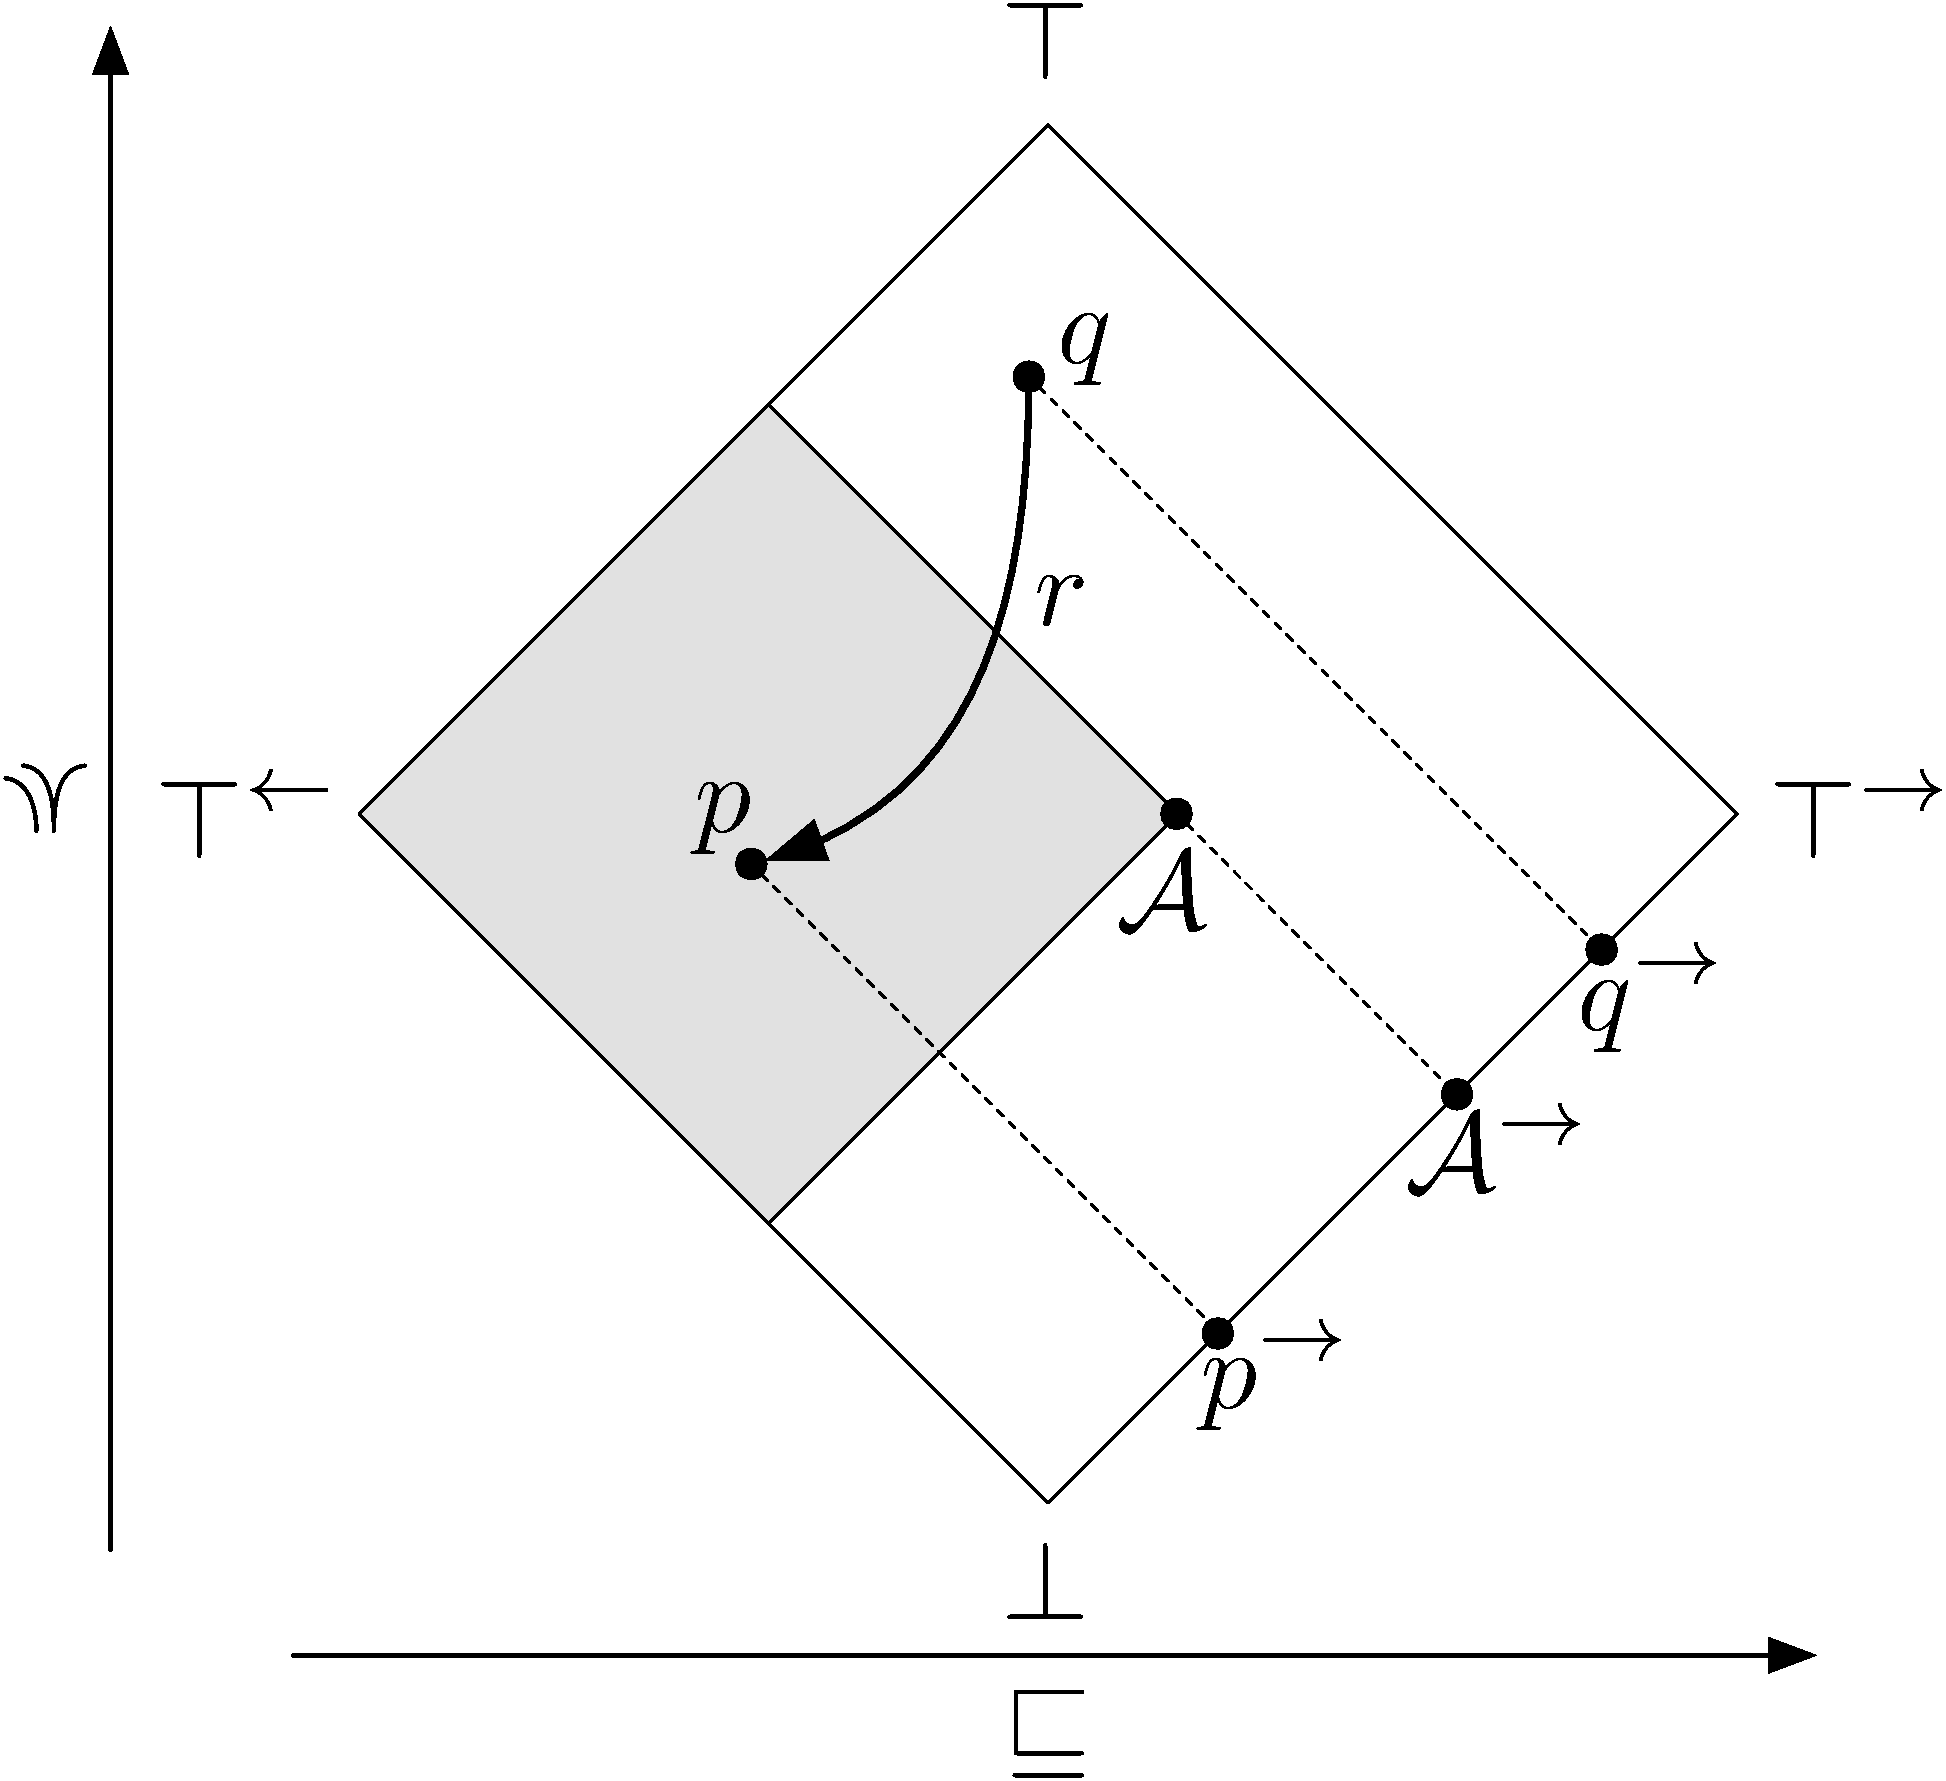
\includegraphics[scale=0.25]{Illustrations/bad-flow.pdf}
    \caption{Information labeled with principal $q$, which previously could not be relabeled as $\Attacker$, can now be relabeled as $p$. This information can, in turn, now be relabeled as $\Attacker$.}
    \label{fig:bad-release}
\end{figure}

\paragraph{Low-equivalence of traces and memories}

\paragraph{Attacker knowledge}
We present our noninterference result using the notion of attacker knowledge \cite{A bunch of Aslan's papers}. The attacker's knowledge is the set of initial memories that could lead to a given observable trace, and a larger knowledge correspond to more uncertainty about the initial memory. Formally, an attacker's knowledge given a trace $t$ produced by expression $\expr$ and the initial set of memories $\globalstore$ is the set
\begin{equation*}
k^n_{\Attacker}(\globalstore, \expr, t) = \left\{ \, \altglobalstore \, \middle\vert \, \globalstore \simeq_{\Attacker} \altglobalstore \wedge \; \gconfig{n}{\emptyenv}{S} \gstepstos[][\Attacker \filtertrace t'] \wedge \; t \simeq_{\Attacker} t' \, \right\}
\end{equation*}
where $S(m) = \config{\altglobalstore(n)}{\llbracket \expr \rrbracket_n(m)}$ and
\begin{equation*}
\llbracket \expr \rrbracket_n(m) =
\begin{cases}
\expr & \text{ if } n = m\\
\termsym & \text{ otherwise }
\end{cases}
\end{equation*}
and $\emptyenv: \Nameset \to \sigma$ represents the initial global environment $\emptyenv(n) = (\bot^{\flowsto}, \varnothing, \nil)$.


Talk about:
\begin{enumerate}
    \item Traces
    \item Good declassifications
    \item Memory and trace low equivalence
    \item Define knowledge
    \item Define TINI
    \item Show the TINI statement
\end{enumerate}